\chapter{Project presentation}

\section{Introduction}
This current chapter is dedicated to giving a global overview of the project.  \\
This part presents the organization, including its problems , its difficulties , and the solution implemented .

\section{Presentation of the host organization  }

\subsection{The host organization introduction }
\begin{figure}[H]
   \centering
    %\includegraphics[scale=0.5]{images/trasfvs.jpg}
    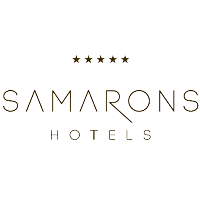
\includegraphics[width=6cm,height=6cm]{images/hotel.png}
    \caption{logo}
    \label{Samarons hotels logo}
\end{figure}
Exuding an aura of refined elegance and unsurpassed luxury, Samarons hotel epitomizes the pinnacle of opulent hospitality. With an unwavering commitment to impeccable service and an array of exclusive amenities, our distinguished establishment stands as a beacon of sophistication and comfort.  

\subsection{Organizational chart}

This is the structure of Samarons hotels :

\begin{enumerate}
\textbf{    \item General Manager:}
Overseeing the entire hotel operations, including the Computer Science department.

\textbf{    \item Computer Science Department:}

\begin{itemize}
\textbf{        \item Chief Technology Officer (CTO):}
Responsible for the overall technology strategy and implementation within the hotel.

        \item \textbf{IT Manager:}
Manages the hotel's IT infrastructure and oversees the Computer Science department's operations.

\textbf{        \item Software Development Team:}

    \begin{itemize}
            \item Development Manager
            \item Software Engineers/Developers
    \end{itemize}

\textbf{        \item Network and Systems Team:}

    \begin{itemize}
            \item Network Manager
            \item System Administrators
    \end{itemize}

\textbf{        \item Database Management Team:}

    \begin{itemize}
            \item Database Manager
            \item Database Administrators
    \end{itemize}

\textbf{        \item IT Support and Help Desk:}

    \begin{itemize}
            \item IT Support Manager
            \item IT Support Specialists
    \end{itemize}

\textbf{        \item Cybersecurity Team:}

    \begin{itemize}
            \item Cybersecurity Manager
            \item Cybersecurity Analysts
    \end{itemize}

\textbf{        \item Digital Marketing and E-Commerce Team:}

    \begin{itemize}
            \item Digital Marketing Manager
            \item E-Commerce Manager
    \end{itemize}

\textbf{        \item Technology Procurement and Vendor Management:}

    \begin{itemize}
            \item Procurement Manager
            \item Vendor Relationship Manager
    \end{itemize}

\end{itemize}

\textbf{    \item Rooms Division:}
Including roles such as Director of Rooms, Front Office Manager, and Housekeeping Manager.

\textbf{    \item Food and Beverage Division:}
Including roles such as Director of Food and Beverage, Executive Chef, Restaurant Manager, and Bar Manager.

\textbf{    \item Sales and Marketing:}
Including roles such as Director of Sales and Marketing, Sales Manager, and Marketing Manager.

\textbf{    \item Finance and Accounting:}
Including roles such as Director of Finance and Accounting Manager.

\textbf{    \item Human Resources:}
Including roles such as Director of Human Resources and Human Resources Manager.

\textbf{    \item Engineering and Maintenance:}
Including roles such as Director of Engineering and Maintenance Manager.

\textbf{    \item Security:}
Including roles such as Director of Security.

\end{enumerate}
 

\section{Existing analysis }

\textbf{1. Online Presence Analysis:}

The current analysis reveals that the hotel in question lacks any online presence, which severely limits its visibility within the competitive hospitality industry. This absence of a website hinders the hotel's ability to promote its services, showcase its amenities, and attract potential guests. Without an online platform, it is challenging for prospective clients to access crucial information such as room rates, available services, and the hotel's location.

\textbf{2. Competitor Analysis:}

A comprehensive study of the competitors in the same category or similar categories highlights that most hotels have well-designed and user-friendly websites. These websites provide features such as online booking, appealing photo galleries, detailed information about rooms and services, and customer testimonials. The online presence of competitors significantly contributes to their brand recognition, reputation, and customer acquisition.

\textbf{3. Reservation Channel Analysis:}

The hotel heavily relies on third-party reservation channels, such as online booking platforms (e.g., Booking.com, Expedia, etc.), due to the lack of its own website. This dependency can lead to high commissions and a loss of control over pricing policies and customer relationships. The absence of a direct reservation channel also limits the hotel's ability to establish a direct connection with its customers, making it challenging to personalize the guest experience and foster customer loyalty.

\textbf{4. Customer Feedback Analysis:}

Customer feedback analysis indicates that many clients face difficulties in obtaining accurate information about the hotel, including pricing, services offered, and room availability. Some guests express a preference for making direct reservations with the hotel instead of using intermediaries.

\textbf{5. Analysis of Potential Benefits:}

Implementing a website for the hotel offers numerous potential benefits, including increased visibility, improved control over pricing and room availability, enhanced guest experience, and the opportunity to establish direct relationships with customers. A well-designed website can also bolster the hotel's credibility and foster trust among potential clients.

 
\subsection{Description of the current situation }

The hotel suffers from a lack of visibility, a loss of control over reservations, and difficulties in establishing a direct relationship with its clientele due to the absence of a structured and effective online presence. The implementation of an optimized website thus represents a key opportunity to improve its competitive position and strengthen its relationship with customers.
\end{itemsize}

\subsection{Critique of the existing situation  }

The lack of an online presence for the hotel poses several significant challenges and drawbacks that hinder its competitiveness and customer reach in the modern digital landscape. Some critical points of critique include:

\begin{enumerate}
{        \item \textbf{Missed Marketing Opportunities:}}
The absence of a dedicated website deprives the hotel of crucial marketing opportunities to showcase its unique offerings, amenities, and services. This lack of visibility limits its ability to reach potential customers who primarily rely on online sources for hotel information and bookings.

\textbf{    \item Limited Customer Engagement:} 
Without a digital platform, the hotel struggles to engage with customers directly and provide personalized services. The inability to establish direct communication channels may lead to missed opportunities for tailored offerings, special promotions, and personalized customer experiences.

\textbf{    \item Dependence on Third-Party Channels:}
Relying solely on third-party booking channels often results in higher commission fees and reduced control over pricing strategies and customer data. This dependency can impact the hotel's revenue and profitability, limiting its ability to implement competitive pricing and tailored promotional campaigns.

\textbf{    \item Competitive Disadvantage:} 
In an industry where online presence is crucial, the hotel's lack of a website places it at a significant competitive disadvantage compared to other hotels that have well-established online platforms. Potential customers may overlook the hotel in favor of competitors with more accessible information and user-friendly booking processes.

\textbf{    \item Diminished Brand Image:}
The absence of a professional website can undermine the hotel's brand image and credibility in the eyes of potential customers. In the absence of an online platform, the hotel may struggle to establish a strong brand identity and may appear outdated or less reputable compared to competitors with robust online presences.

\textbf{    \item Inadequate Information Access:} 
Prospective guests may face challenges in obtaining comprehensive and accurate information about the hotel's amenities, room availability, and pricing. This lack of transparency and accessibility can deter potential customers and lead to missed business opportunities.

\end{enumerate}

\subsection{Proposed solution  }

To address the existing challenges and improve the hotel's competitiveness, the following solutions are proposed:

\begin{enumerate}
{        \item \textbf{Website Development:}}
Develop a user-friendly, visually appealing, and informative website that showcases the hotel's unique offerings, amenities, and services. Implement an intuitive user interface and ensure seamless navigation for an enhanced user experience.

\textbf{    \item Online Reservation System:}
Integrate a secure and efficient online reservation system directly on the hotel's website. This system should enable guests to check room availability, view pricing, and make direct bookings without the need for third-party booking platforms, thus reducing commission fees and improving the hotel's revenue stream.
\end{enumerate}
 
\section{Conclusion}
In this study,  the lack of an online presence for the hotel has significantly constrained its ability to compete effectively in the digital era of the hospitality industry. This absence has resulted in missed marketing opportunities, limited customer engagement, and a competitive disadvantage compared to other hotels with robust online platforms. Relying solely on third-party booking channels has also led to higher commission fees and reduced control over pricing strategies.
That's why we proposed the solution of a reservation and description website.